% Options for packages loaded elsewhere
\PassOptionsToPackage{unicode}{hyperref}
\PassOptionsToPackage{hyphens}{url}
%
\documentclass[
]{article}
\usepackage{lmodern}
\usepackage{amssymb,amsmath}
\usepackage{ifxetex,ifluatex}
\ifnum 0\ifxetex 1\fi\ifluatex 1\fi=0 % if pdftex
  \usepackage[T1]{fontenc}
  \usepackage[utf8]{inputenc}
  \usepackage{textcomp} % provide euro and other symbols
\else % if luatex or xetex
  \usepackage{unicode-math}
  \defaultfontfeatures{Scale=MatchLowercase}
  \defaultfontfeatures[\rmfamily]{Ligatures=TeX,Scale=1}
\fi
% Use upquote if available, for straight quotes in verbatim environments
\IfFileExists{upquote.sty}{\usepackage{upquote}}{}
\IfFileExists{microtype.sty}{% use microtype if available
  \usepackage[]{microtype}
  \UseMicrotypeSet[protrusion]{basicmath} % disable protrusion for tt fonts
}{}
\makeatletter
\@ifundefined{KOMAClassName}{% if non-KOMA class
  \IfFileExists{parskip.sty}{%
    \usepackage{parskip}
  }{% else
    \setlength{\parindent}{0pt}
    \setlength{\parskip}{6pt plus 2pt minus 1pt}}
}{% if KOMA class
  \KOMAoptions{parskip=half}}
\makeatother
\usepackage{xcolor}
\IfFileExists{xurl.sty}{\usepackage{xurl}}{} % add URL line breaks if available
\IfFileExists{bookmark.sty}{\usepackage{bookmark}}{\usepackage{hyperref}}
\hypersetup{
  pdftitle={Practical 06 BSG: Association analysis},
  pdfauthor={Lovro Katalinic and Ivan Almer},
  hidelinks,
  pdfcreator={LaTeX via pandoc}}
\urlstyle{same} % disable monospaced font for URLs
\usepackage[margin=1in]{geometry}
\usepackage{color}
\usepackage{fancyvrb}
\newcommand{\VerbBar}{|}
\newcommand{\VERB}{\Verb[commandchars=\\\{\}]}
\DefineVerbatimEnvironment{Highlighting}{Verbatim}{commandchars=\\\{\}}
% Add ',fontsize=\small' for more characters per line
\usepackage{framed}
\definecolor{shadecolor}{RGB}{248,248,248}
\newenvironment{Shaded}{\begin{snugshade}}{\end{snugshade}}
\newcommand{\AlertTok}[1]{\textcolor[rgb]{0.94,0.16,0.16}{#1}}
\newcommand{\AnnotationTok}[1]{\textcolor[rgb]{0.56,0.35,0.01}{\textbf{\textit{#1}}}}
\newcommand{\AttributeTok}[1]{\textcolor[rgb]{0.77,0.63,0.00}{#1}}
\newcommand{\BaseNTok}[1]{\textcolor[rgb]{0.00,0.00,0.81}{#1}}
\newcommand{\BuiltInTok}[1]{#1}
\newcommand{\CharTok}[1]{\textcolor[rgb]{0.31,0.60,0.02}{#1}}
\newcommand{\CommentTok}[1]{\textcolor[rgb]{0.56,0.35,0.01}{\textit{#1}}}
\newcommand{\CommentVarTok}[1]{\textcolor[rgb]{0.56,0.35,0.01}{\textbf{\textit{#1}}}}
\newcommand{\ConstantTok}[1]{\textcolor[rgb]{0.00,0.00,0.00}{#1}}
\newcommand{\ControlFlowTok}[1]{\textcolor[rgb]{0.13,0.29,0.53}{\textbf{#1}}}
\newcommand{\DataTypeTok}[1]{\textcolor[rgb]{0.13,0.29,0.53}{#1}}
\newcommand{\DecValTok}[1]{\textcolor[rgb]{0.00,0.00,0.81}{#1}}
\newcommand{\DocumentationTok}[1]{\textcolor[rgb]{0.56,0.35,0.01}{\textbf{\textit{#1}}}}
\newcommand{\ErrorTok}[1]{\textcolor[rgb]{0.64,0.00,0.00}{\textbf{#1}}}
\newcommand{\ExtensionTok}[1]{#1}
\newcommand{\FloatTok}[1]{\textcolor[rgb]{0.00,0.00,0.81}{#1}}
\newcommand{\FunctionTok}[1]{\textcolor[rgb]{0.00,0.00,0.00}{#1}}
\newcommand{\ImportTok}[1]{#1}
\newcommand{\InformationTok}[1]{\textcolor[rgb]{0.56,0.35,0.01}{\textbf{\textit{#1}}}}
\newcommand{\KeywordTok}[1]{\textcolor[rgb]{0.13,0.29,0.53}{\textbf{#1}}}
\newcommand{\NormalTok}[1]{#1}
\newcommand{\OperatorTok}[1]{\textcolor[rgb]{0.81,0.36,0.00}{\textbf{#1}}}
\newcommand{\OtherTok}[1]{\textcolor[rgb]{0.56,0.35,0.01}{#1}}
\newcommand{\PreprocessorTok}[1]{\textcolor[rgb]{0.56,0.35,0.01}{\textit{#1}}}
\newcommand{\RegionMarkerTok}[1]{#1}
\newcommand{\SpecialCharTok}[1]{\textcolor[rgb]{0.00,0.00,0.00}{#1}}
\newcommand{\SpecialStringTok}[1]{\textcolor[rgb]{0.31,0.60,0.02}{#1}}
\newcommand{\StringTok}[1]{\textcolor[rgb]{0.31,0.60,0.02}{#1}}
\newcommand{\VariableTok}[1]{\textcolor[rgb]{0.00,0.00,0.00}{#1}}
\newcommand{\VerbatimStringTok}[1]{\textcolor[rgb]{0.31,0.60,0.02}{#1}}
\newcommand{\WarningTok}[1]{\textcolor[rgb]{0.56,0.35,0.01}{\textbf{\textit{#1}}}}
\usepackage{graphicx,grffile}
\makeatletter
\def\maxwidth{\ifdim\Gin@nat@width>\linewidth\linewidth\else\Gin@nat@width\fi}
\def\maxheight{\ifdim\Gin@nat@height>\textheight\textheight\else\Gin@nat@height\fi}
\makeatother
% Scale images if necessary, so that they will not overflow the page
% margins by default, and it is still possible to overwrite the defaults
% using explicit options in \includegraphics[width, height, ...]{}
\setkeys{Gin}{width=\maxwidth,height=\maxheight,keepaspectratio}
% Set default figure placement to htbp
\makeatletter
\def\fps@figure{htbp}
\makeatother
\setlength{\emergencystretch}{3em} % prevent overfull lines
\providecommand{\tightlist}{%
  \setlength{\itemsep}{0pt}\setlength{\parskip}{0pt}}
\setcounter{secnumdepth}{-\maxdimen} % remove section numbering

\title{Practical 06 BSG: Association analysis}
\author{Lovro Katalinic and Ivan Almer}
\date{Hand-in: 21/12/2020}

\begin{document}
\maketitle

In this practical we perform association tests for a binary disease
indicator and a genetic polymorphism. Resolve the following exercise in
groups of two students. Perform the computations and make the graphics
that are asked for in the practical below. Take care to give each graph
a title, and clearly label x and y axes, and to answer all questions
asked. You can write your solution in a word or Latex document and
generate a pdf file with your solution. Alternatively, you may generate
a solution pdf file with Markdown. You can use R packages MASS,
genetics, data.table and others for the computations. Take care to
number your answer exactly as in this exercise, preferably by copying
each requested item into your solution. Upload your solution to the web
page of the course at raco.fib.upc.edu no later than the hand-in date.

\begin{Shaded}
\begin{Highlighting}[]
\KeywordTok{library}\NormalTok{(MASS)}
\KeywordTok{library}\NormalTok{(genetics)}
\end{Highlighting}
\end{Shaded}

\begin{verbatim}
## Loading required package: combinat
\end{verbatim}

\begin{verbatim}
## 
## Attaching package: 'combinat'
\end{verbatim}

\begin{verbatim}
## The following object is masked from 'package:utils':
## 
##     combn
\end{verbatim}

\begin{verbatim}
## Loading required package: gdata
\end{verbatim}

\begin{verbatim}
## gdata: Unable to locate valid perl interpreter
## gdata: 
## gdata: read.xls() will be unable to read Excel XLS and XLSX files
## gdata: unless the 'perl=' argument is used to specify the location of a
## gdata: valid perl intrpreter.
## gdata: 
## gdata: (To avoid display of this message in the future, please ensure
## gdata: perl is installed and available on the executable search path.)
\end{verbatim}

\begin{verbatim}
## gdata: Unable to load perl libaries needed by read.xls()
## gdata: to support 'XLX' (Excel 97-2004) files.
\end{verbatim}

\begin{verbatim}
## 
\end{verbatim}

\begin{verbatim}
## gdata: Unable to load perl libaries needed by read.xls()
## gdata: to support 'XLSX' (Excel 2007+) files.
\end{verbatim}

\begin{verbatim}
## 
\end{verbatim}

\begin{verbatim}
## gdata: Run the function 'installXLSXsupport()'
## gdata: to automatically download and install the perl
## gdata: libaries needed to support Excel XLS and XLSX formats.
\end{verbatim}

\begin{verbatim}
## 
## Attaching package: 'gdata'
\end{verbatim}

\begin{verbatim}
## The following object is masked from 'package:stats':
## 
##     nobs
\end{verbatim}

\begin{verbatim}
## The following object is masked from 'package:utils':
## 
##     object.size
\end{verbatim}

\begin{verbatim}
## The following object is masked from 'package:base':
## 
##     startsWith
\end{verbatim}

\begin{verbatim}
## Loading required package: gtools
\end{verbatim}

\begin{verbatim}
## Loading required package: mvtnorm
\end{verbatim}

\begin{verbatim}
## 
\end{verbatim}

\begin{verbatim}
## NOTE: THIS PACKAGE IS NOW OBSOLETE.
\end{verbatim}

\begin{verbatim}
## 
\end{verbatim}

\begin{verbatim}
##   The R-Genetics project has developed an set of enhanced genetics
\end{verbatim}

\begin{verbatim}
##   packages to replace 'genetics'. Please visit the project homepage
\end{verbatim}

\begin{verbatim}
##   at http://rgenetics.org for informtion.
\end{verbatim}

\begin{verbatim}
## 
\end{verbatim}

\begin{verbatim}
## 
## Attaching package: 'genetics'
\end{verbatim}

\begin{verbatim}
## The following objects are masked from 'package:base':
## 
##     %in%, as.factor, order
\end{verbatim}

\begin{Shaded}
\begin{Highlighting}[]
\KeywordTok{library}\NormalTok{(data.table)}
\end{Highlighting}
\end{Shaded}

\begin{verbatim}
## 
## Attaching package: 'data.table'
\end{verbatim}

\begin{verbatim}
## The following objects are masked from 'package:gdata':
## 
##     first, last
\end{verbatim}

The file rs394221.dat contains genotype information, for cases and
controls, of polymorphism rs394221, which is presumably related to
Alzheimer's disease. Load the data file into the R environment.

\begin{enumerate}
\def\labelenumi{\arabic{enumi}.}
\tightlist
\item
  (1p) What is the sample size? What is the number of cases and the
  number of controls? Construct the contingency table of genotype by
  case/control status.
\end{enumerate}

\begin{Shaded}
\begin{Highlighting}[]
\NormalTok{data <-}\StringTok{ }\KeywordTok{fread}\NormalTok{(}\StringTok{'rs394221.dat'}\NormalTok{, }\DataTypeTok{data.table=}\OtherTok{FALSE}\NormalTok{, }\DataTypeTok{header =} \OtherTok{FALSE}\NormalTok{)}
\NormalTok{n <-}\StringTok{ }\KeywordTok{nrow}\NormalTok{(data)}
\NormalTok{ncases <-}\StringTok{ }\KeywordTok{sum}\NormalTok{(data[,}\DecValTok{2}\NormalTok{] }\OperatorTok{==}\StringTok{ 'case'}\NormalTok{)}
\NormalTok{ncontrol <-}\StringTok{ }\NormalTok{n }\OperatorTok{-}\StringTok{ }\NormalTok{ncases}

\KeywordTok{cat}\NormalTok{(}\KeywordTok{paste}\NormalTok{(}\StringTok{'Number of rows:'}\NormalTok{, n, }\StringTok{'}\CharTok{\textbackslash{}n}\StringTok{'}\NormalTok{))}
\end{Highlighting}
\end{Shaded}

\begin{verbatim}
## Number of rows: 1167
\end{verbatim}

\begin{Shaded}
\begin{Highlighting}[]
\KeywordTok{cat}\NormalTok{(}\KeywordTok{paste}\NormalTok{(}\StringTok{'Number of cases:'}\NormalTok{, ncases, }\StringTok{'}\CharTok{\textbackslash{}n}\StringTok{'}\NormalTok{))}
\end{Highlighting}
\end{Shaded}

\begin{verbatim}
## Number of cases: 509
\end{verbatim}

\begin{Shaded}
\begin{Highlighting}[]
\KeywordTok{cat}\NormalTok{(}\KeywordTok{paste}\NormalTok{(}\StringTok{'Number of controls:'}\NormalTok{, ncontrol, }\StringTok{'}\CharTok{\textbackslash{}n}\StringTok{'}\NormalTok{))}
\end{Highlighting}
\end{Shaded}

\begin{verbatim}
## Number of controls: 658
\end{verbatim}

\begin{Shaded}
\begin{Highlighting}[]
\KeywordTok{head}\NormalTok{(data)}
\end{Highlighting}
\end{Shaded}

\begin{verbatim}
##   V1      V2
## 1 Mm    case
## 2 Mm control
## 3 mm    case
## 4 mm control
## 5 mm control
## 6 MM    case
\end{verbatim}

\begin{enumerate}
\def\labelenumi{\arabic{enumi}.}
\setcounter{enumi}{1}
\tightlist
\item
  (1p) Explore the data by plotting the percentage of cases as a
  function of the genotype, ordering the latter according to the number
  of M alleles. Which allele increases the risk of the disease?
\end{enumerate}

\begin{Shaded}
\begin{Highlighting}[]
\NormalTok{mms <-}\StringTok{ }\KeywordTok{sum}\NormalTok{(data[,}\DecValTok{2}\NormalTok{] }\OperatorTok{==}\StringTok{ 'case'} \OperatorTok{&}\StringTok{ }\NormalTok{data[,}\DecValTok{1}\NormalTok{] }\OperatorTok{==}\StringTok{ 'mm'}\NormalTok{)}
\NormalTok{Mms <-}\StringTok{ }\KeywordTok{sum}\NormalTok{(data[,}\DecValTok{2}\NormalTok{] }\OperatorTok{==}\StringTok{ 'case'} \OperatorTok{&}\StringTok{ }\NormalTok{data[,}\DecValTok{1}\NormalTok{] }\OperatorTok{==}\StringTok{ 'Mm'}\NormalTok{)}
\NormalTok{MMs <-}\StringTok{ }\KeywordTok{sum}\NormalTok{(data[,}\DecValTok{2}\NormalTok{] }\OperatorTok{==}\StringTok{ 'case'} \OperatorTok{&}\StringTok{ }\NormalTok{data[,}\DecValTok{1}\NormalTok{] }\OperatorTok{==}\StringTok{ 'MM'}\NormalTok{)}
\NormalTok{number_of_alleles <-}\StringTok{ }\KeywordTok{c}\NormalTok{(}\DecValTok{0}\NormalTok{,}\DecValTok{1}\NormalTok{,}\DecValTok{2}\NormalTok{)}
\NormalTok{genotypes_distr <-}\StringTok{ }\KeywordTok{c}\NormalTok{(mms, Mms, MMs)}\OperatorTok{/}\NormalTok{ncases}

\KeywordTok{plot}\NormalTok{(number_of_alleles, genotypes_distr, }\DataTypeTok{main=}\StringTok{"Percentage of cases by genotype"}\NormalTok{, }\DataTypeTok{xlab=}\StringTok{"Number of M alleles"}\NormalTok{, }\DataTypeTok{ylab=}\StringTok{"Frequency of genotypes in cases"}\NormalTok{)}
\KeywordTok{lines}\NormalTok{(number_of_alleles, genotypes_distr, }\DataTypeTok{col=}\StringTok{"gray"}\NormalTok{)}
\end{Highlighting}
\end{Shaded}

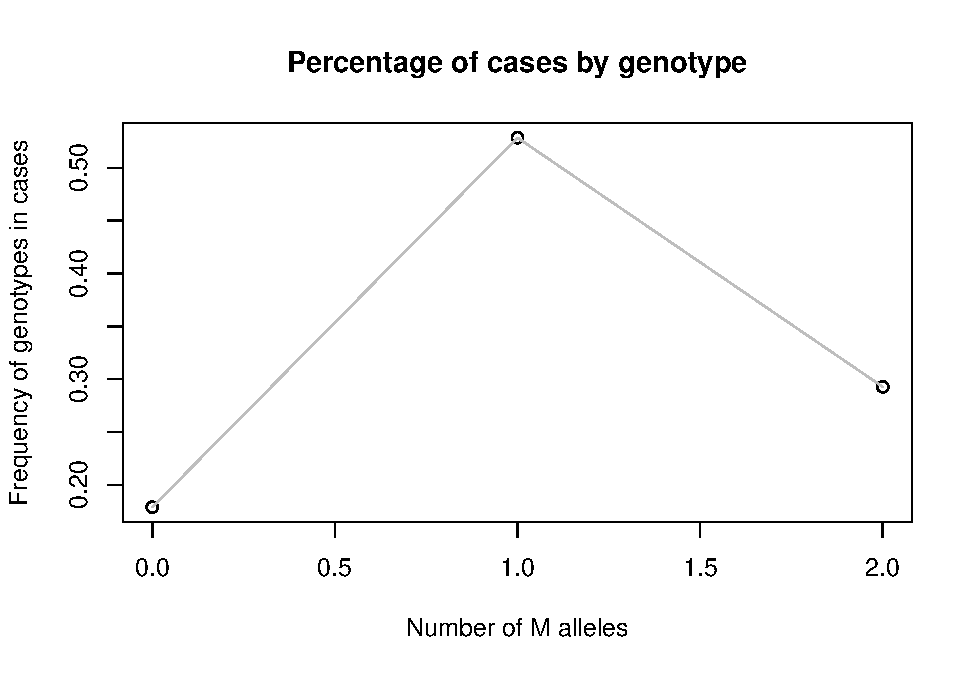
\includegraphics{P062020_Association_analysis_files/figure-latex/second-1.pdf}

Considering this plot, we can say that genotype \emph{Mm} increases the
risk of desease. If we compare alleles, we can observe that there are
more cases with allele \emph{M} than \emph{m} .

\begin{enumerate}
\def\labelenumi{\arabic{enumi}.}
\setcounter{enumi}{2}
\tightlist
\item
  (2p) Test for equality of allele frequencies in cases and controls by
  doing an alleles test. Report the test statistic, its reference
  distribution, and the p-value of the test. Is there evidence for
  different allele frequencies?
\end{enumerate}

\begin{Shaded}
\begin{Highlighting}[]
\NormalTok{mcases <-}\StringTok{ }\DecValTok{2}\OperatorTok{*}\KeywordTok{sum}\NormalTok{(data[,}\DecValTok{2}\NormalTok{] }\OperatorTok{==}\StringTok{ 'case'} \OperatorTok{&}\StringTok{ }\NormalTok{data[,}\DecValTok{1}\NormalTok{] }\OperatorTok{==}\StringTok{ 'mm'}\NormalTok{) }\OperatorTok{+}\StringTok{ }\KeywordTok{sum}\NormalTok{(data[,}\DecValTok{2}\NormalTok{] }\OperatorTok{==}\StringTok{ 'case'} \OperatorTok{&}\StringTok{ }\NormalTok{data[,}\DecValTok{1}\NormalTok{] }\OperatorTok{==}\StringTok{ 'Mm'}\NormalTok{)}
\NormalTok{Mcases <-}\StringTok{ }\DecValTok{2}\OperatorTok{*}\KeywordTok{sum}\NormalTok{(data[,}\DecValTok{2}\NormalTok{] }\OperatorTok{==}\StringTok{ 'case'} \OperatorTok{&}\StringTok{ }\NormalTok{data[,}\DecValTok{1}\NormalTok{] }\OperatorTok{==}\StringTok{ 'MM'}\NormalTok{) }\OperatorTok{+}\StringTok{ }\KeywordTok{sum}\NormalTok{(data[,}\DecValTok{2}\NormalTok{] }\OperatorTok{==}\StringTok{ 'case'} \OperatorTok{&}\StringTok{ }\NormalTok{data[,}\DecValTok{1}\NormalTok{] }\OperatorTok{==}\StringTok{ 'Mm'}\NormalTok{)}
\NormalTok{mcontrol <-}\StringTok{ }\DecValTok{2}\OperatorTok{*}\KeywordTok{sum}\NormalTok{(data[,}\DecValTok{2}\NormalTok{] }\OperatorTok{==}\StringTok{ 'control'} \OperatorTok{&}\StringTok{ }\NormalTok{data[,}\DecValTok{1}\NormalTok{] }\OperatorTok{==}\StringTok{ 'mm'}\NormalTok{) }\OperatorTok{+}\StringTok{ }\KeywordTok{sum}\NormalTok{(data[,}\DecValTok{2}\NormalTok{] }\OperatorTok{==}\StringTok{ 'control'} \OperatorTok{&}\StringTok{ }\NormalTok{data[,}\DecValTok{1}\NormalTok{] }\OperatorTok{==}\StringTok{ 'Mm'}\NormalTok{)}
\NormalTok{Mcontrol <-}\StringTok{ }\DecValTok{2}\OperatorTok{*}\KeywordTok{sum}\NormalTok{(data[,}\DecValTok{2}\NormalTok{] }\OperatorTok{==}\StringTok{ 'control'} \OperatorTok{&}\StringTok{ }\NormalTok{data[,}\DecValTok{1}\NormalTok{] }\OperatorTok{==}\StringTok{ 'MM'}\NormalTok{) }\OperatorTok{+}\StringTok{ }\KeywordTok{sum}\NormalTok{(data[,}\DecValTok{2}\NormalTok{] }\OperatorTok{==}\StringTok{ 'control'} \OperatorTok{&}\StringTok{ }\NormalTok{data[,}\DecValTok{1}\NormalTok{] }\OperatorTok{==}\StringTok{ 'Mm'}\NormalTok{)}

\NormalTok{allele_freq <-}\StringTok{ }\KeywordTok{rbind}\NormalTok{(}\KeywordTok{c}\NormalTok{(mcases, Mcases), }\KeywordTok{c}\NormalTok{(mcontrol, Mcontrol))}
\KeywordTok{colnames}\NormalTok{(allele_freq) <-}\StringTok{ }\KeywordTok{c}\NormalTok{(}\StringTok{"m"}\NormalTok{,}\StringTok{"M"}\NormalTok{)}
\KeywordTok{rownames}\NormalTok{(allele_freq) <-}\StringTok{ }\KeywordTok{c}\NormalTok{(}\StringTok{"Cases"}\NormalTok{, }\StringTok{"Control"}\NormalTok{)}

\KeywordTok{chisq.test}\NormalTok{(allele_freq,}\DataTypeTok{correct=}\OtherTok{FALSE}\NormalTok{)}
\end{Highlighting}
\end{Shaded}

\begin{verbatim}
## 
##  Pearson's Chi-squared test
## 
## data:  allele_freq
## X-squared = 13.797, df = 1, p-value = 0.0002037
\end{verbatim}

As the chi-squared statistic of 13.797 which corresponds to p-value
0.0002037 exceeds the critical value, we reject the null hypothesis and
conclude that the allele frequencies are biased at 95\% significance
level. We say that there is enough evidence for different allele
frequencies.

\begin{enumerate}
\def\labelenumi{\arabic{enumi}.}
\setcounter{enumi}{3}
\tightlist
\item
  (2p) Which are the assumptions made by the alleles test? Perform and
  report any additional tests you consider adequate to verify the
  assumptions. Do you think the assumptions of the alleles test are met?
\end{enumerate}

The assumptions made by chi-squared test are \emph{random sampling},
\emph{sufficiently large size of sample}, \emph{expected cell count
greater than 5} and \emph{independence of the observations}.*

\begin{Shaded}
\begin{Highlighting}[]
\DecValTok{000}
\end{Highlighting}
\end{Shaded}

\begin{verbatim}
## [1] 0
\end{verbatim}

\begin{enumerate}
\def\labelenumi{\arabic{enumi}.}
\setcounter{enumi}{4}
\tightlist
\item
  (2p) Perform the Armitage trend test for association between disease
  and number of M alleles. Report the test statistic, its reference
  distribution and the p-value of the test. Do you find evidence for
  association?
\item
  (4p) Test for association between genotype and disease status by a
  logistic regression of disease status on genotype, treating the latter
  as categorical. Do you find significant evidence for association?
  Which allele increase the risk for the disease? Give the odds ratios
  of the genotypes with respect to base line genotype mm. Provide 95\%
  confidence intervals for these odds ratios.
\end{enumerate}

\end{document}
